% !TEX root = SystemTemplate.tex
\chapter{Design  and Implementation}
 This section describes the design details for the overall system as well as individual major components. As a user, you will have a good understanding of the implemetation details without having to look into the code. Note that the
 code to generate test cases is only run if there is a -g cammond line switch is specified after the directory to test is entered.

 Here is an overview of the algorithm:

\begin{itemize}
  \item Determine if there is a .cpp file in the root directory, if so it is used to generate test cases
  \item Create a vector containing every subdirectory in program folder
  \item Change to directory where student subdirectories are located
  \item Step through each directory in the directory vector and determine if it contains tests or student source code
  \item Create a vector containing the name each student's source and one containing the path to their source code
  \item Create a vector containing all of the test cases
  \item While the source code vector is not empty
  \item Compile the program
  \item Determine if the student passes the critical test cases, if not stop testing
  \item Run code against tests in the test vecotor
  \item Count whether the program passed or failed test case
  \item If it failed with a normal diff, test if it passes with presentation errors
  \item Change back to home directory 
  \item Write log file containing percentage of tests passed and final grade
  \item Write students results to summary file
\end{itemize}


\section{Traversing Subdirectories (Sprint 2)}

\subsection{Technologies  Used}
The dirent.h library is used for traversing subdirectories.

\subsection{Design Details}

\begin{lstlisting}

bool change_dir(string dir_name)
{
    string path;
    if(chdir(dir_name.c_str()) == 0) 
    {
        path = get_pathname();
        return true;
    }
    return false;
}

bool is_dir(string dir)
{
    struct stat file_info;
    stat(dir.c_str(), &file_info);
    if ( S_ISDIR(file_info.st_mode) ) 
        return true;
    else 
        return false;
}
\end{lstlisting}

\section{Running the Program Using Test Cases (Sprint 2)}

\subsection{Technologies  Used}
The software was designed in the Linux Environment.


\subsection{Design Details}


\begin{lstlisting}
int run_file(string cpp_file, string test_case) //case_num
{
    //create .out file name
    string case_out(case_name(test_case, "out"));

    //set up piping buffers
    string buffer1("");
    string buffer2(" &>/dev/null < ");
    string buffer3(" > ");

    // "try using | "
    //construct run command, then send to system
    //./<filename> &> /dev/null  < case_x.tst > case_x.out
    buffer1 += cpp_file + buffer2 + test_case + buffer3 + case_out;
    system(buffer1.c_str());

    //0 = Fail, 1 = Pass
    return result_compare(test_case);
}
\end{lstlisting}

\section {Testing to Allow for Presentation Errors}

\subsection {Technologies Used}
This set of function relies on the string, cmath, and fstream libraries to test if two
files match, allowing for presentation errors.

\subsection {Design Details}
This software checks if two files match, allowing for presentation errors.  These presentation
errors include, ignoring capitilization errors, if two words start and end with the same letters
then they are counted as matching, if two words have the same letters but the wrong
order they are counted as matching, if a number would round to the correct value it is
considered correct.  Below is the code for comparing two files.

\begin{lstlisting}
bool cmpFiles(string s1, string s2)
{
    ifstream file1, file2;
    string in1, in2;

    file1.open(s1.c_str());
    file2.open(s2.c_str());
    if( !file1 || !file2 )
    {
        cout << "Files to be compared could not be opened" << endl;
        file1.close();
        file2.close();
        return false;
    }

    while (file1 >> in1)
    {
        if (file2 >> in2)
        {
            if(in1 != in2)
            {
                if(isNumber(in1))
                {
                    if(isNumber(in2))
                    {
                        //both inputs are numbers
                        //if in2 doesn't round to in1 file is wrong
                        if (!cmpNum(in1,in2))
                        {
                            //file failed
                            file1.close();
                            file2.close();
                            return false;
                        }
                    }
                    else
                    {
                        //in1 is number, in2 is not, file is wrong
                        //file failed
                        file1.close();
                        file2.close();
                        return false;
                    }
                }
                else
                {
                    if(isNumber(in2))
                    {
                        //in1 is a string in2 is a number, file is wrong
                        //file failed
                        file1.close();
                        file2.close();
                        return false;
                    }
                    else
                    {
                        //in1 and in2 are strings
                        //if in1 and in2 don't match with presentation errors
                        if (!cmpString(in1,in2))
                        {
                            //file failed
                            file1.close();
                            file2.close();
                            return false;
                        }
                    }
                }
            }
        }
        else
        {
            //file is missing information
            //file failed
            file1.close();
            file2.close();
            return false;
        }
    }

    //if the second file has additonal information
    if (file2 >> in2)
    {
        //file failed
        file1.close();
        file2.close();
        return false;
    }
    file1.close();
    file2.close();
    return true;
}
\end{lstlisting}

\section {Test Generation}
The test generation in this product allows for generation of test files for integer, floating point, and string values
along with generating tests for menu driven testing.

\subsection {Technologies Used}
The test generation relies on the cmath and fstream libraries, to allow for random generation and actually
writing the files respectively.

\subsection {Design Details}
The following is code only for the menu-driven test geneation, though all the other generation types
have similar code, the menu-driven test generate all three kinds of inputs, int, floating, and string.

\begin{lstlisting}
void generateMenuTestCases( string goldenName , string specName )
{
    int numTestCases;   // the number of test cases to generate, the user will
                        //   the number
    float temp;         // used for input
    ifstream specFile;  // file stream of the .spec file
    ofstream outFile;   // file stream of the current .tst file being writen to
    string pathName;    // path to the directory containing the generated .tst
                        //   files
    string homePath = get_pathname();   // the path to the current directory
    ostringstream convert;  // used in converting ints to strings for creating
                            //   .tst files
    string command;     // string used to create command line arguments
    string testString;  // string used in the creation of random strings
    int max;            // the maximum range of generated digits, user will 
                        //   input this
    int min;            // the minimum range of generated digits, user will
                        //   input this
    float tempRand;     // used in the generation of random floating point
                        //   numbers
    int stringSize;     // the length of random strings, user will input this
    int i, j;
    
    tempRand = 0;
    
    // print out message saying that spec file was detected
    cout << "Spec file detected, creating menu test cases" << endl;
    
    //open the spec file
    specFile.open( specName.c_str() );
    
    if ( specFile.is_open() == false )
    {
        cout << "Unable to open spec file" << endl;
        return;
    }
    
    // prompt for number of test cases to be used and get it
    cout << "Please enter the number of test cases to be generated: ";
    do
    {
        cin >> numTestCases;
        cout << endl;
        if( numTestCases <= 0 )
        {
            cout << "Enter a number greater then 0: ";
        }
        
    }while( numTestCases <= 0 );
    
    cout << "Enter the max for ints, floats, and doubles: ";
    cin >> max;
    cout << endl;
    
    cout << "Enter the min for ints, floats, and doubles: ";
    cin >> min;
    cout << endl;
    
    cout << "Enter the length of the strings: ";
    cin >> stringSize;
    cout << endl;
    
    
    for( i = 0 ; i < numTestCases ; i++ )
    {
        // open up output file
        convert << i;
        pathName = homePath + "/test/GENERATED_TEST_FILE_" + convert.str() + ".tst";
        outFile.open( pathName.c_str() );
        
        // set specFile to beginning 
        specFile.seekg( 0 , ios::beg );
        
        // output a test case of 0 for first menu option
        outFile << "0" << endl;
        
        specFile >> command;
        while( !specFile.eof() )
        {
            if ( command == "int" )
            {
                // output a random int
                outFile << rand() % (max - min) + min << endl;
            }
            else if ( command == "float" || command == "double" )
            {
                // output a random float
                while ( tempRand == 0)
                {
                    tempRand = float (rand()) / float (RAND_MAX);
                    if ( tempRand == 1)
                        tempRand--;
                }
                    outFile << tempRand + fmod(rand(), (float)(max - min)) + (float)min << endl;
                    tempRand = 0;
            }
            else if ( command == "string" )
            {
                // ouput a random string
                for( int j = 0; j < stringSize; j++)
                {
                    //generate  random character.
                    char temp = (char) (rand() % 26 + 97);
                    testString += temp;
                }
                //write the string to the test file
                outFile << testString << endl;
            }
            else
            {
                // output the menu option to the tst
                outFile << command;
            }
            
            
            specFile >> command;
        }
        generate_ans( goldenName, pathName);
        outFile.close();
    }
    
    
    return;
}
\end{lstlisting}


\section {System Diagram}
The following are system diagrams for first, the overall program, and the second a more detailed
one of how to determine if two files match with presentation errors.

\begin {figure}[tbh]
\begin {center}
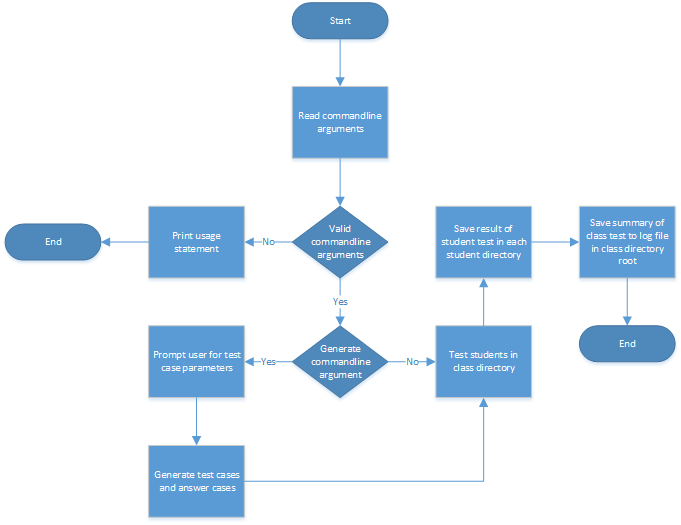
\includegraphics[width=1\textwidth]{./SystemDiagram}
\end{center}
\caption{System Diagram\label{systemdiagram}}
\end{figure}

\begin{figure}[tbh]
\begin{center}
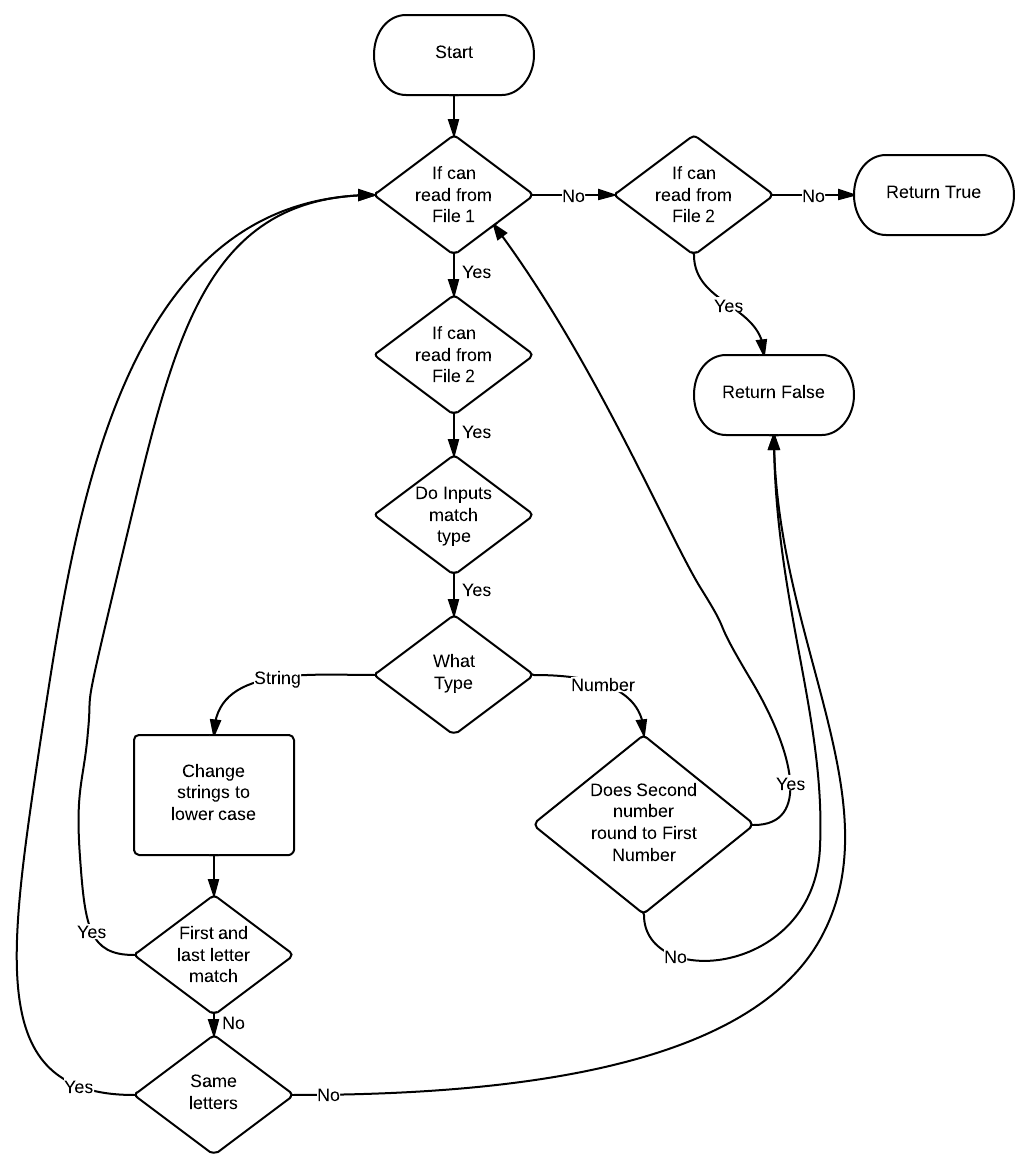
\includegraphics[width=1\textwidth]{./SystemDiagram2}
\end{center}
\caption{System Diagram for Testing to Allow for Presentation Errors\label{systemdiagram2}}
\end{figure}

